% #####################################################################################################################################################################################
\hoofdstuk{Requirements}
% #####################################################################################################################################################################################

Even though a general goal and vision are important for guiding which direction the application goes towards, they must be broken down into smaller, more concrete and measurable objectives.. These are called requirements and are used to determine the project’s progress and whether it was completed successfully or not. The following requirements were deduced from the project’s problem and objective:

\begin{itemize}
    \item{\textbf{The application must be able to locate the license plate within an image.} \\
        One of the most important functionalities of the application, without this requirement most of the following requirements can not be accomplished. Must find a plate within an image where a plate is present and ignore everything else if no license plate is present.        
    }

    \item{\textbf{The application must be able to recognize the text displayed on the license plate.} \\
        The other requirement which ties the whole application together. Once the plate has been located, the text contained in the plate must be parsed so the application possesses information to work further. 
    }

    \item{\textbf{The application must be able to retrieve a list of license plates from a designated website.} \\
         For the application to be able to provide useful information about a certain vehicle, it must have information about stole vehicles to match the recognize plate text against. Therefore it must be able to retrieve that information from the place where it is available, in the case a website.
    }

    \item{\textbf{The application must be able to match the recognised text in the license plate to the retrieved list.} \\
        The application must be able to match the retrieved information of stolen vehicles with the recognised text.
    }

    \item{\textbf{The application must be not save any information/images longer than necessary.} \\
        As to minimise the chance any privacy law will be broken, the application will not save any form of data which might be used to identify someone. The reason for this is explained in a later chapter.
    }
\end{itemize}

% #####################################################################################################################################################################################
\hoofdstuk {Methodology}
% #####################################################################################################################################################################################

Before starting the development, the methods must be found which will be used to find viable ways of solving the problems presented by the requirements and how to implement them once the correct solutions have been found. For this reason some time was first spent searching for possible research and development methods, and suitable technologies. In the end the following choices were made.

\paragraaf{Research method}

The method applied for researching the problems of this project and its possible solutions is called \emph{literature review}. This method consists of researching what has already been published, which might be in the form of scientific or engineering papers, journals, thesis, etc., by accredited scientists, scholars or engineers concerning this assignment's topics. 
This method is applied for searching for potential algorithms which can be used to solve the problems created by the requirements. Once a group of the most suitable algorithms has been found, the best one must be chosen and the reasoning for this choice must be explained. When the choice has been made, the algorithm is then implemented using the chosen development method.

\paragraaf{Development method}

This project will be developed using the \emph{Iterative Application Development} (IAD) method. This development method works by dividing the project into smaller `sub-projects', called \emph{cycles}, and incrementing them to past cycles, which will ultimately lead to a complete system. Each cycle consists of three phases, which can be repeated multiple times if necessary, called \emph{iterations}. These iterations are: \emph{definition}, \emph{development} and \emph{deployment}.

During the definition phase the goals, limitations and conditions for the current cycle are examined and described. If a previous cycle has been completed, it will be evaluated during this phase. This phase is intended for thinking towards the completion of the project and to achieve a more clear picture of the system as a whole.
After defining the objective for the new cycle, the software will be developed. After finishing, the software is then integrated with the software developed in the previous cycles and becomes therefore part of the general project.

This method of software development brings multiple benefits: The complexity of the project is decreased by breaking down the problem into smaller chunks, which allows for faster and more concrete results and makes it therefore easier to get better feedback or to solve critical bottlenecks by being able to discuss them at the end of each cycle. The project development also becomes more flexible by having the possibility to review the requirements and strategies every cycle.

Each cycle lasts 2 weeks and at the end of each cycle the evaluation of the past cycle and the objective for the coming cycle will be discussed with the organisation's mentor.

% #####################################################################################################################################################################################
\hoofdstuk{Algorithms}
% #####################################################################################################################################################################################

When reasoning about what kind of main algorithms would be necessary to develop the application and after researching which software could be used to develop the application, the problem was then broken down into two different categories: localising the plate within an image, because it is a very specific problem which requires a specific algorithm to solve, and parsing the text within the plate, which is a broader case and there are available libraries which can be promptly used to solve this problem. After this realisation and researching the possibilities, the following choices were made.

\paragraaf{Plate localization}

When searching for possible algorithms which make it possible to find license plates in an image, two main types came forth from the research: feature detection and edge detection. 

The feature detection algorithms work by finding so called \emph{features} in a image, which are used to recognize the first image within a second one. These features are segments of an image which must be uncommon, as to reduce the possibility of retrieving a false positive when applying the algorithm, and also consist of something which can be objectively described to a computer. Because of these requirements, the features extracted from images are usually corners since corners usually only match themselves when compared to other segments in an image. This opposed to flat surfaces or lines, which may appear multiple times in multiple places in the same image. Because this algorithm focuses on detecting the uniqueness of an image and using those attributes to detect themselves in different images, it is difficult to use feature detection for the recognition of license plates for the reason that every license plate contains unique text. The considerable collection of diverse shapes that exist in the Latin alphabet create false positives which are often detected in random and incorrect locations. One possible approach to use this algorithm would be by creating a feature database of every possible alphanumeric character and then finding the highest concentration of text as a possible location. 

The other possible algorithm is mostly based on edge detection. This kind of algorithm works by applying an edge detection filter to a grey scale version of the image where the car is present. This creates a binary image where the edges of every shape present in the image are displayed. Because of the nature of one of the characteristics common to every license plate, which is the presence of text, an area with a high density of edges is created. Although license plates are not the only objects which might have such a property, e.g. a fence, it is the most common one which might be encountered while driving. By applying this filter to find horizontal edges it is possible to find the vertical location of the plate and then vice-versa to find the horizontal location and by extension the plate itself. Due to little information on the performance of the feature detection algorithm and a healthy amount of information regarding this one, this algorithm was chosen.

This algorithm was implemented using Open Computer Vision (OpenCV) library which is a library that contains optimized state-of-the-art computer vision algorithms. This library is maintained by Intel, a company known for its mathematical knowledge, is completely free, as in beer and as in freedom, and has an Android version. Because of these reasons and prior experience working with this library, OpenCV was chosen. Although the application was implemented using this library, this thesis explains the algorithms usage in a general, OpenCV-agnostic way as to be easier to understand the algorithms without the need for the library.


\paragraaf{Text recognition}

Text recognition is a specific problem which will only vary slightly from project to project, which usually means it has to be trained to recognize a different font or the text to be recognised has a special orientation, e.g. vertical or diagonal. There are libraries which have specifically this functionality along with enough customizability to adjust the library to the specific needs of the project. There is for this reason no need to create an own text recognition algorithm.
From the available options in OCR technology, the Tesseract Optical Character Recognition (OCR) was chosen because it is maintained by Google, a company known for its OCR technology, and it is one of the most accurate free OCR libraries available and also has an Android version. It was chosen because no there are no other free library available which can deliver the same type of results. The implementation of the text recognition is Tesseract specific because, as op



% #####################################################################################################################################################################################
\hoofdstuk{Design}
% #####################################################################################################################################################################################

Before the application can be built, some sort of blueprint must be created where the functionality, the flow, and a variety of other specifications are incorporated and described. This is called the design of the application and it outlines what each component does, how they are interconnected, and the reasoning behind each choice.

\paragraaf{Privacy}

Privacy has always been an hot topic within the computer science circle of professions with computers becoming faster each year and all sort of algorithms being created which have the potential to invade the privacy of thousands if not millions of people. As of the writing of this thesis, a chain of events have gotten this kind of controversy to a new all-time high. 
To prevent that this application will ever create any privacy concerns, some research was done on the Dutch privacy law of personal information as of 2014. According to this law, it is only possible to transgress if, while collecting license plate information, the following three requirements are met. The information must be:

\begin{enumerate}
    \item{\textbf{personal information} \\
        The information gathered must qualify as personal information. This means the information must directly link to a certain person, e.g. phone number, address or name but also pictures of people's faces. The only instance which has access to the personal information linked to a license plate is the \textit{Rijksdienst voor het Wegverkeer}, which is a government instance, and therefore the only instance which would have to comply to the privacy law. It is possible to access that information through their services, but you need the information's owner's permission and have to pay a fee, which means accidental transgression of the law impossible is.
    }

    \item{\textbf{processed} \\
        Processing information is a very broad concept, which can be anything from using the information for a website or just matching it against a database.
    }

    \item{\textbf{saved in a file} \\
        This can be a simple spreadsheet or a full-fledged database.
    }
\end{enumerate}

This application will only meet the second point, which means it will not violate the Dutch privacy law. To add some additional certainty, the application will only save the license plate information for as long as necessary, will not save any pictures taken after they have been processed and the user will not have direct access to that information.

\paragraaf{Application}
The top-level flow of the system consists of three individual components: the website where the license plate information of stole cars is available, this android application which using the information from the website tries to match that information with captured video images, and a central server where, if a match has been found between the previous two stages, the match information is sent to. A diagram of this flow can be seen in Figure \ref{fig:top-level}.

\begin{figure}[ht]
    \centering
    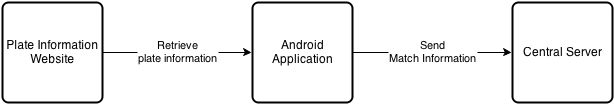
\includegraphics[width=0.8\textwidth]{plaatjes/top-down}
    \caption{Top-level diagram.}
    \label{fig:top-level}
\end{figure}%

Although all those three components are part of the whole system, this project only focuses on the application itself. A flowchart illustrating the general design and flow of the application is displayed in Figure \ref{fig:architecture}. Within an Android application all components run in the same thread by default, which is also known as the `main thread', and is identified in the flowchart as `UI' because it is used mainly to regulate all the processes related to the user interface. One of those processes, and also one of the most fundamental running in this thread, is the process which captures images from the device's camera. The process captures image frames at a set rate in order to avoid the unnecessary capture of very similar images and, because image processing algorithms consist of a large number of calculations and therefore might take a long time to finish, to avoid overwhelming the application with too many frames. These images are then pushed into a buffer, called `Frames buffer', where they are kept until they are able to be processed. For the same reasons the camera only captures frames at a specific rate, this buffer has a limit of how many frames can be stored within but with the intention of only preserving images which are as recent as possible, before a new frame is added the oldest remaining frame in the buffer is removed. This process runs until the application is terminated.

As explained before, image processing is rather heavy and it is necessary to use every tool available to increase the application's performance. One of these tools is multi-threading and apart from the UI thread this application uses two other kinds of threads, up to a total of four threads which is also the number of physical cores in the used device and therefore gives every thread a dedicated core. The processes called `Find bands' and `Find plate' use a type of thread called a \emph{One-Call Thread}, which are threads used for a short period of time and only run when called. The other kind of thread is called a \emph{Permanent thread}. This type of thread is started during the initiation of the application, runs parallel to the UI thread and lives as long as the application itself. This process is responsible for checking whether the bands and plates buffers have available items and for calling the respective processes to process them. Further, if a plate is found then this thread applies text recognition to retrieve the displayed text and tries to match it with the database entries. If there is a match, the application will save the plate information for a defined amount of time, the default being 30 minutes, to prevent sending the same of very similar information about the whereabouts of the vehicle every time the application recognizes the plate. Furthermore, the plate's information will be bundled together with the current location of the smartphone, the current time and the confidence of the recognition. This bundled message will then be sent to a central server where it can then be distributed to the correct authorities. After this has been done or if there wasn't a match, the system starts again from the beginning.


\begin{figure}[ht]
    \centering
    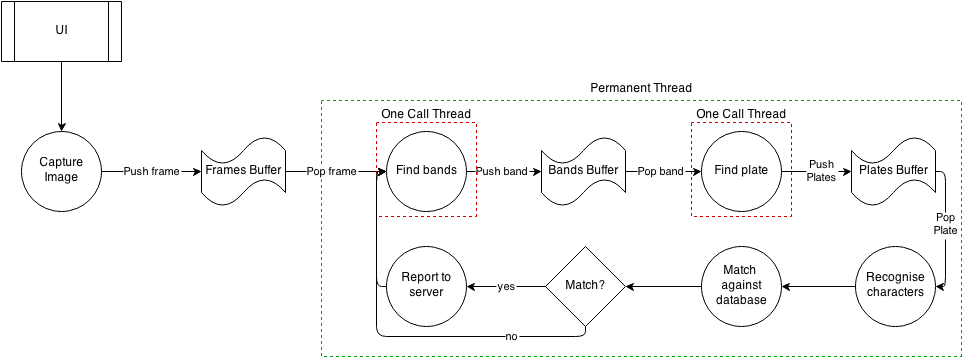
\includegraphics[width=\textwidth]{plaatjes/architecture-RoadEye-parallel}
    \caption{Application flow diagram.}
    \label{fig:architecture}
\end{figure}%

% #####################################################################################################################################################################################
\hoofdstuk{Implementation}
% #####################################################################################################################################################################################

The application consists of three main components: the algorithms for finding the vertical and horizontal locations of the license plates, and the text recognition component. Both localization algorithms are based on the work of Martinský Ondrej \cite{ondrej2007algorithmic}, with some slight modifications, which are explained in the following chapters, to fit the requirements of this application. 
The algorithms use the car in Figure \ref{fig:car-source} to demonstrate how they work.

\begin{figure}[ht]
    \centering
    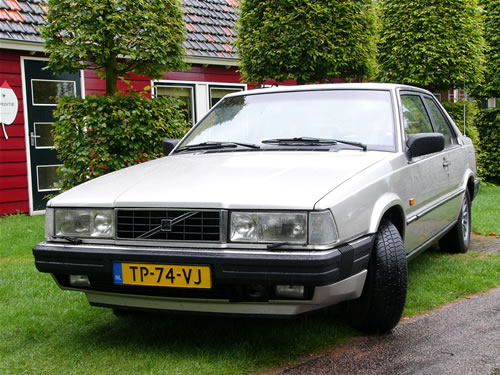
\includegraphics[width=0.40\textwidth]{plaatjes/car}
    \caption{Source car image. \cite{source-car-fig}}
    \label{fig:car-source}
\end{figure}%

\paragraaf{Bands}

The first step to locating a license plate is to find its vertical location, which also known as a band. Using one of the most characteristic features of a Dutch license plate, which is its yellow colour and can be seen on Figure \ref{fig:dutch-plate}, it is possible to reduce the area of the image where the license plate might be located through the application of colour segmentation. 

\begin{figure}[ht]
    \centering
    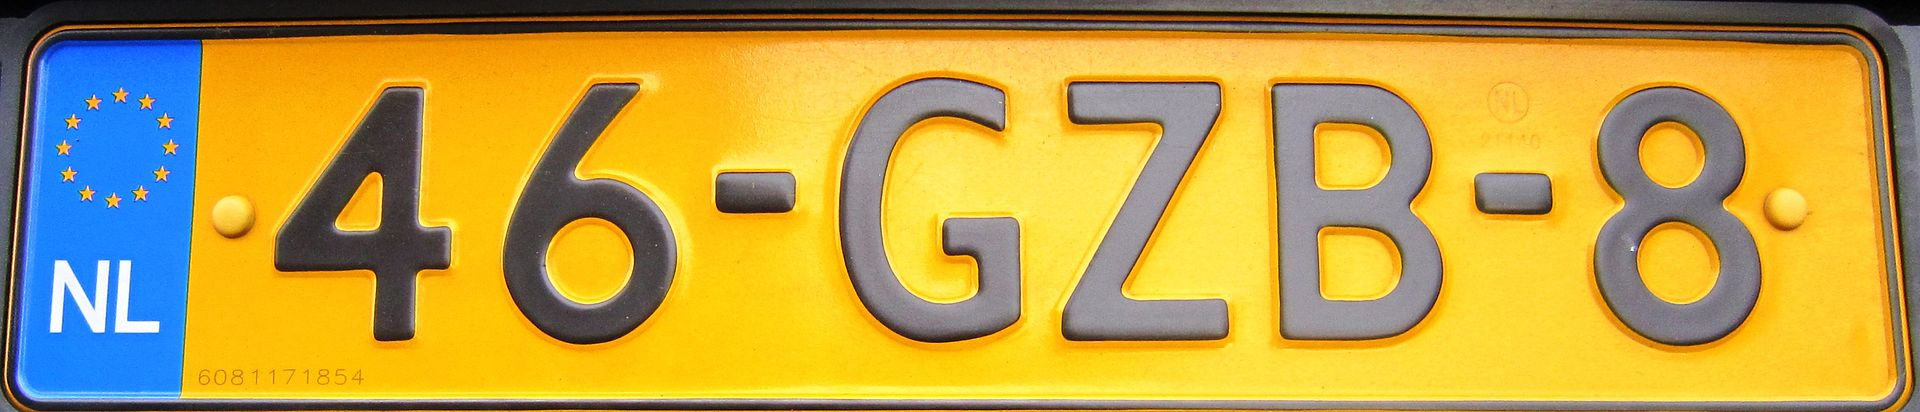
\includegraphics[width=0.3\textwidth]{plaatjes/dutch-plate}
    \caption{Dutch license plate. \cite{dutch-license-fig}}
    \label{fig:dutch-plate}
\end{figure}

Colour segmentation consists of fetching only the areas of an image which fall within a specified colour range and is usually used on an image which uses the HSV colour space representation. As seen in Figure \ref{fig:hsv}, HSV stands for Hue, Saturation, and Value and it is a way of representing colours on a computer. This in contrast to the most widely used colour space, the RGB colour space (Red, Green, Blue) which uses a combination of those very colours to represent a specific colour. The HSV colour space on the other hand uses the H-value to represent the pixel's colour and is defined in degrees (0$^{\circ}$ - 360$^{\circ}$), the S-value to represent how bleak or how colourful the pixel is and is defined with a percentage (0\% - 100\%), and the V-value to represent its brightness or darkness and is defined the same way as the saturation. This provides a system where it is simple to choose a colour range for the colour segmentation algorithm and is also the standard system for these kind of operations. The range chosen for the license plate lays between 40$^{\circ}$ and 50$^{\circ}$, which is broad enough to take into consideration the deviations in the colour of the plate caused by shadows and reflections.

\begin{figure}[ht]
    \centering
    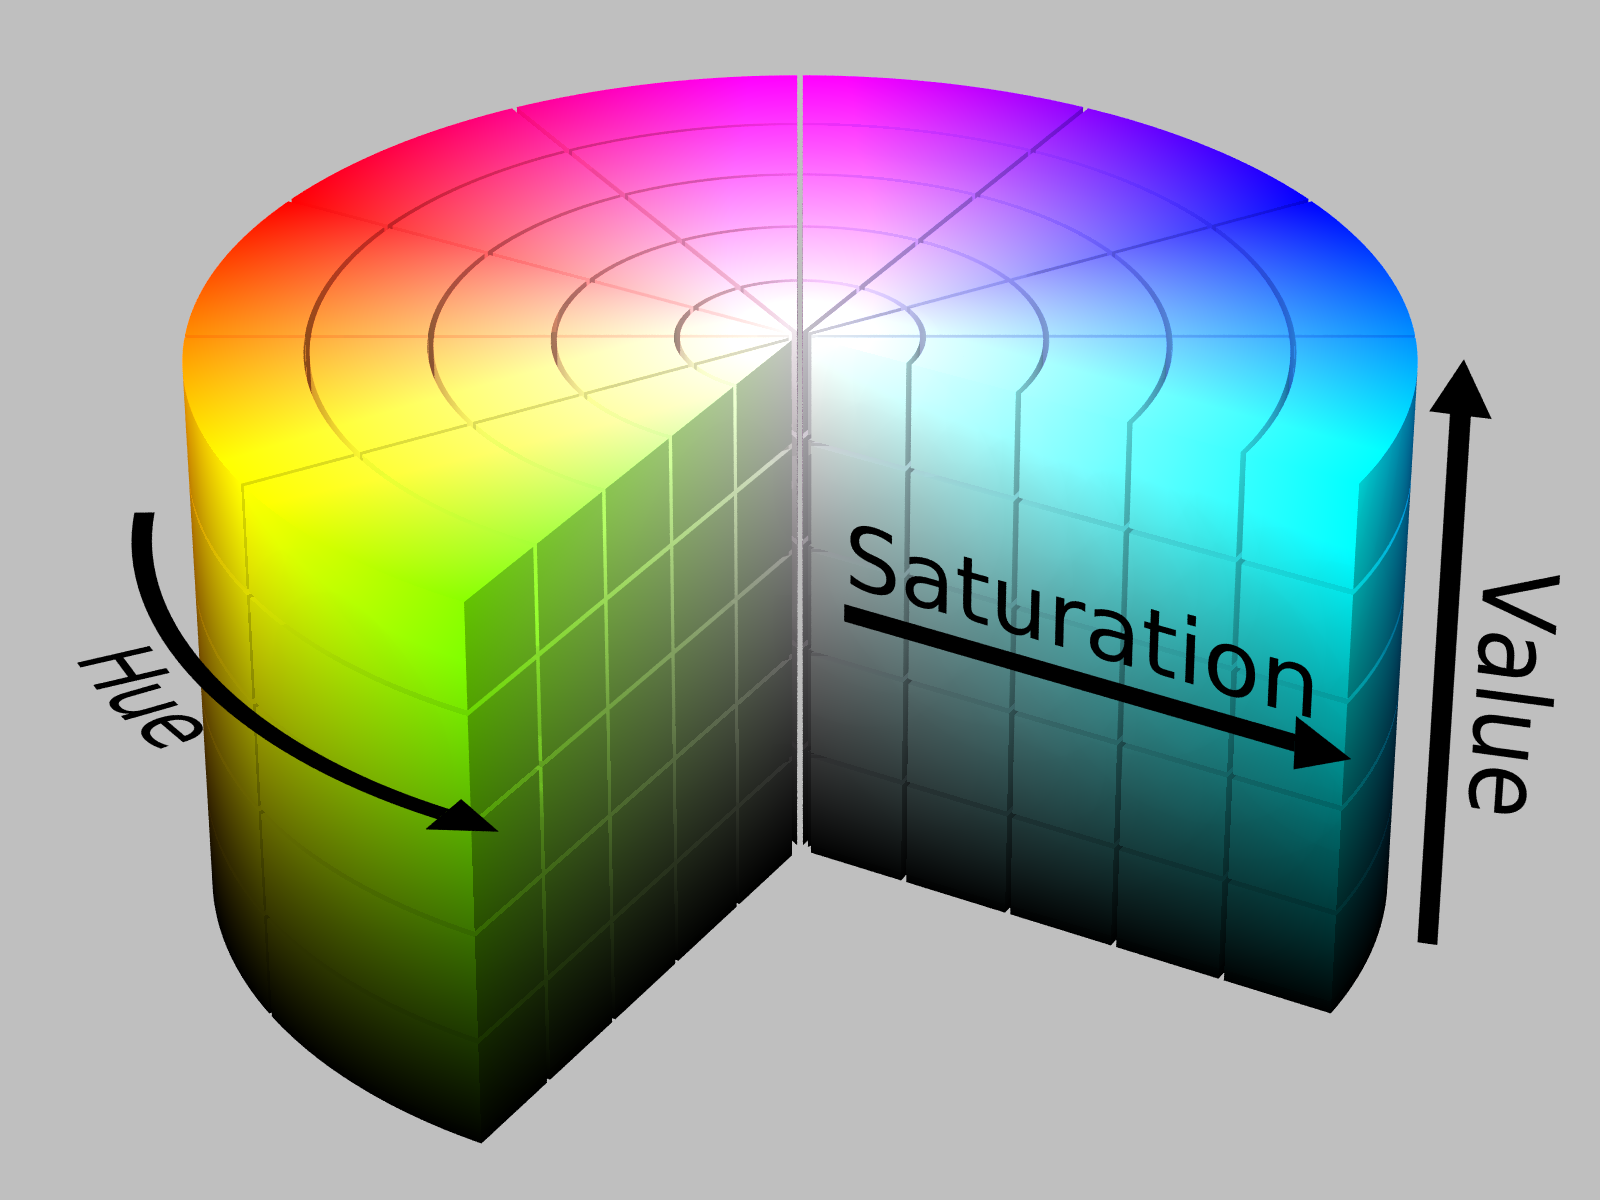
\includegraphics[width=0.3\textwidth]{plaatjes/hsv}
    \caption{HSV colour space. \cite{hsv-fig}}
    \label{fig:hsv}
\end{figure}

As a result of segmenting the yellow colour from the source image, the image in Figure \ref{fig:color-segmented} is created, where the plate's location is quite visible. Often the segmented image also contains speckles from various small objects present in the image. These speckles are also visible in the previously mentioned image and might cause incorrect results when trying to locate the plate. To prevent this, a morphological closing operation \cite{morphclose} is performed. This operation works by dilating the image, which actually dilates its background and therefore removes small objects but also reduces the area of the plate, followed by eroding the dilated image, which does the inverse of the previous operation and returns the plate to its original size while the small objects are still gone. Further, because there are such things as yellow cars and other yellow objects, an extra step must be taken to decrease the chance of finding random objects. This is accomplished by making use of a characteristic of text and by extension of license plates, which is a high number of edges. By applying an edge detection algorithm, in this case the Sobel operator \cite{sobel} was used and its output is visible in Figure \ref{fig:edge-detected}, we still get a visible area where the plate is located but in case the source image contained large yellow areas, these areas are now mostly gone.

Once that is done, the application can start analysing the previous image for the license plate's possible location. This is done by summing up the intensity of every pixel on each row and therefore creating a graph where the density of edges on each row is displayed. Before making any decisions concerning the plate's location on the graph, a filter must be applied to the data to remove unwanted data and increase the desired area slightly which is necessary for a later stage. This filter is called a \emph{mean-filter} and works by summing up the values of a specific number of the previous and next data values, in the case of this application seven values are used, with the current value and diving it by the total number of values. The results in the `smooth' graph displayed in Figure \ref{fig:possible-bands}. The next step and last step is finding the potential plate areas and this is done by searching for a number of the highest peaks in the graph, with three being the default. The algorithm tries to find multiple possible locations in case an object in the image happens to have a higher edge density than the plate, and therefore increasing the chance of still finding it. The way the application finds peaks is by finding the highest value in the data set and then searching for the right and left boundary of the peak by iterating towards its respective side until it finds a value which is equal to or smaller than 10\% of the peak's value. The coordinates of both boundaries are then saved and the area in between both coordinates is made equal to zero, or \emph{zeroised}. By rinsing and repeating this process for the chosen number of times, the bands displayed on Figure \ref{fig:possible-bands} are found. 

\begin{figure}[ht]
        \centering
        \begin{subfigure}{0.33\textwidth}
            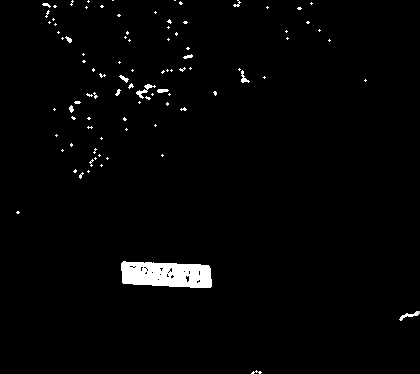
\includegraphics[width=\textwidth]{plaatjes/yellow-segment}
            \caption{Colour segmentation.}
            \label{fig:color-segmented}
        \end{subfigure}%
        ~ 
        \begin{subfigure}{0.33\textwidth}
            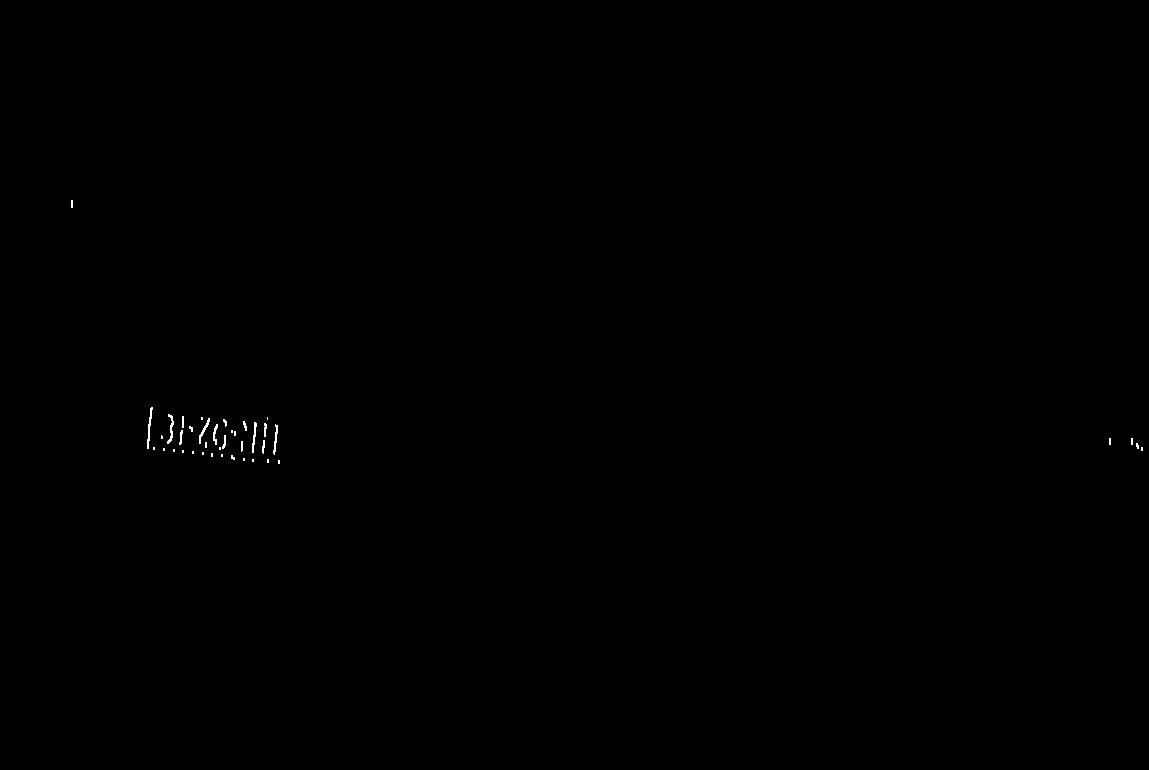
\includegraphics[width=\textwidth]{plaatjes/edge-detection}
            \caption{Edge detection.}
            \label{fig:edge-detected}
        \end{subfigure}%

        \begin{subfigure}{0.5\textwidth}
            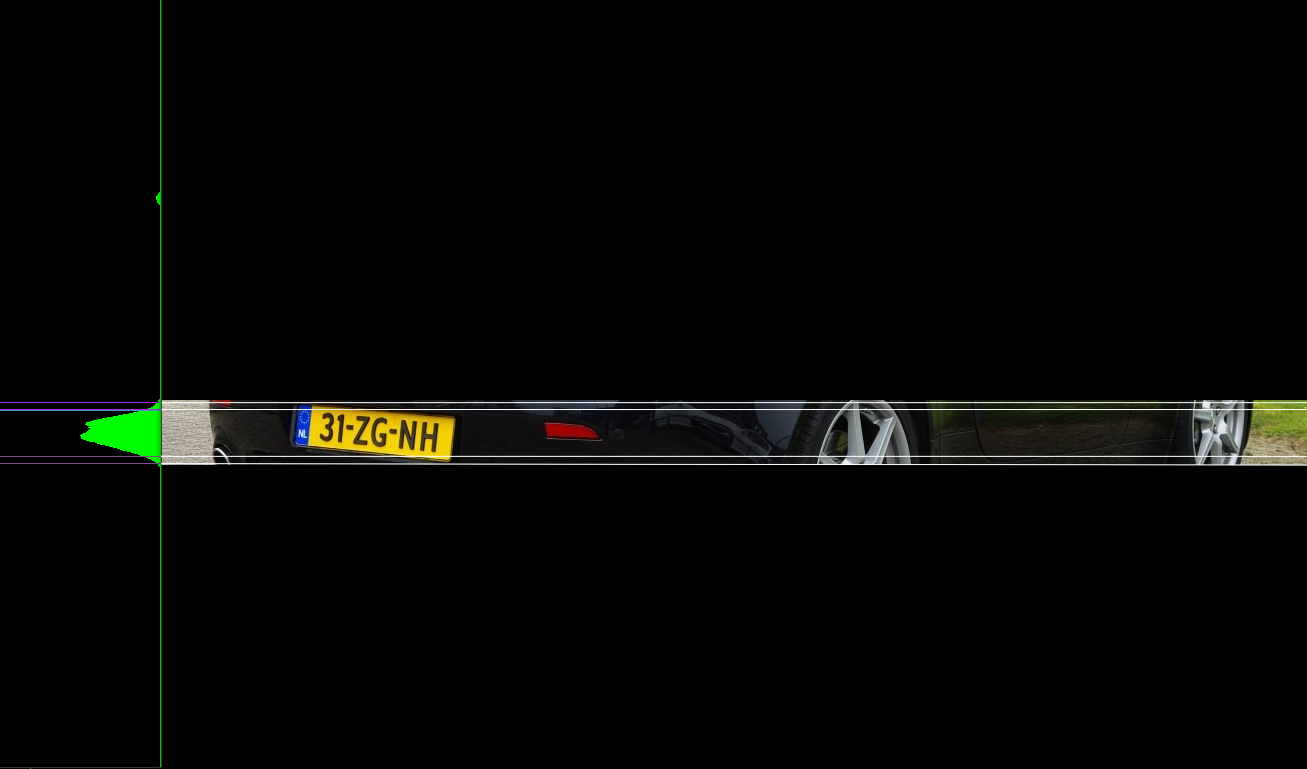
\includegraphics[width=\textwidth]{plaatjes/3-peaks}
            \caption{Possible band(s).}
            \label{fig:possible-bands}
        \end{subfigure}%

        \caption{Phases from band localization.}
        \label{fig:find-band}
\end{figure}

\paragraaf{Plates}

After finding the bands, these can be further processed to find the exact location of the plate. Using the binary version of the band's image, a graph can be generated just like before, but instead of summing up all values on each row, the values of each column are now summed. Once the graph has been created, the mean-filter is also applied for the same reason as before. Using the filtered data the plate is then located by searching for the largest cluster of peaks, as shown in Figure \ref{fig:band-cropped}, which are equivalent to the letters on the plate. The algorithm works by iterating the graph until a data cluster is found, from which the algorithm then saves the start coordinate and keeps iterating the remainder of the graph until it reaches the end of the current cluster. The size of the cluster is then saved and after repeating this process for every data cluster present in the graph, the largest one is chosen as the plate's location. 

\begin{figure}[ht]
    \centering
    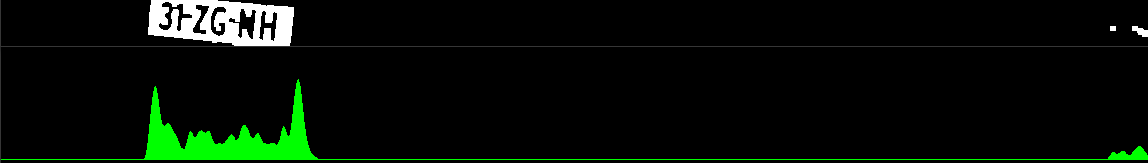
\includegraphics[width=0.5\textwidth]{plaatjes/plate-graph}
    \caption{Horizontal localisation of the plate.}
    \label{fig:band-cropped}
\end{figure}

This gives an image of the plate with a rather larger border of undesired parts of the image, as shown in Figure \ref{fig:skewed-plate}. The reason for this is that depending on the angle at which the image was captured at, the plate might be skewed and the text won't therefore be at a 90$^{\circ}$ angle. This makes it difficult for the OCR software to recognize the text properly. To correct the skewness the bounding box of the plate must be calculated, which is a quadrangle that surrounds the plate's area and from where its four vertices can be retrieved. The box can be seen in Figure \ref{fig:skewed-bounding-box}. Using these points, the angle at which the plate is skewed can then be calculated and the image can then be de-skewed using the warp perspective algorithm \cite{warpperspective} as displayed in Figure \ref{fig:rotated-plate}. 

Finally, only a few last steps are necessary to complete the localisation and processing of the plate before the OCR software takes over. Using the de-skewed plate, a binary image must then be created to allow for the removal of unwanted artefacts still present on the image, e.g. borders. The binary image is created by applying a threshold algorithm onto a greyscale version of the plate, which converts every pixel with an intensity value above a certain threshold to a black pixel and everything else to white. The used threshold algorithm is an adaptive threshold algorithm, which gets its name because of its ability to adapt the threshold value of a pixel according to the neighbouring pixels. In this case the algorithm calculates the mean value of the sum of the pixels around the threshold pixel. This gives a better result than using a fixed value, because the lighting condition is not the same on every image, or a threshold algorithm like Otsu's method \cite{otsu} which requires a distinct difference between foreground and background, which is not always available in the case of a license plate. After applying the threshold algorithm, a binary image is created containing the background in white while the text and eventually some artefacts are in black. The last step left to take is to discriminate the text from everything else and therefore creating an image fit for text recognition. This is accomplished by applying a contour finding algorithm \cite{suzuki}, which finds the outline of every item in the image. By using only the contours which are enclosed within another contour and in turn do not contain other contours within themselves, as is the case of the letters' contours as they are located within the contour of the license plate and contain no further contours inside them. This is possible because the contours algorithm creates a hierarchy list of every contour and whether that contour has a parent and/or child. Once the correct contours have been found they are then drawn on another image, which can be seen in Figure \ref{fig:contour-text}.

\begin{figure}[ht]
        \centering
        \begin{subfigure}{0.33\textwidth}
            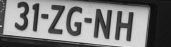
\includegraphics[width=\textwidth]{plaatjes/skewed-plate}
            \caption{Skewed plate.}
            \label{fig:skewed-plate}
        \end{subfigure}%
        ~ 
        \begin{subfigure}{0.33\textwidth}
            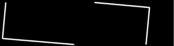
\includegraphics[width=\textwidth]{plaatjes/skewed-plate-box}
            \caption{Bounding box of the plate.}
            \label{fig:skewed-bounding-box}
        \end{subfigure}%
        ~ 
        \begin{subfigure}{0.33\textwidth}
            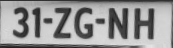
\includegraphics[width=\textwidth]{plaatjes/rotated-plate}
            \caption{De-skewed plate.}
            \label{fig:rotated-plate}
        \end{subfigure}%

        \begin{subfigure}{0.33\textwidth}
            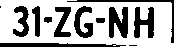
\includegraphics[width=\textwidth]{plaatjes/remove-border-plate}
            \caption{Threshold of plate.}
            \label{fig:threshold-plate}
        \end{subfigure}%
        ~
        \begin{subfigure}{0.33\textwidth}
            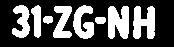
\includegraphics[width=\textwidth]{plaatjes/contour-text}
            \caption{Contours of text.}
            \label{fig:contour-text}
        \end{subfigure}%

        \caption{Phases from the plate de-skewing process.}
        \label{fig:deskewing-plate}
\end{figure}

% Although the results seen in the previous images are quite clear, depending on the angle the original image was taken, it is possible that the characters are slanted. This creates situations when the OCR software cannot recognize the character properly and might even confuse the character for a different one, causing a false positive. To circumvent this problem, the angle at which the character is slanted must be calculated and rectified. This can be done using an Principal Component Analyser (PCA) algorithm. This kind of algorithm is used to find a linear pattern within a dataset and if that dataset happens to be a character, it calculates the direction it is ``pointing'' to. Using that information the angle a which the character is slanted can be calculated. In Figure \ref{fig:pca-line} an example is shown of how a PCA algorithm works. To exemplify how this whole process would apply to a plate, the image on Figure \ref{fig:skewed-car} would be used as a source image.

% \begin{figure}[ht]
%     \centering
%     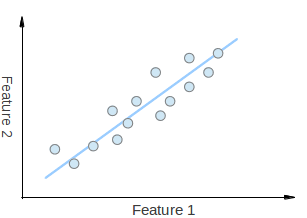
\includegraphics[width=0.4\textwidth]{plaatjes/pca_line}
%     \caption{PCA linear pattern. \cite{pca-line-fig}}
%     \label{fig:pca-line}
% \end{figure}%

% Using the angle determined with the PCA algorithm, a shear transformation can then be applied to remove the inclination angle. Shear transformations are specifically used to add or remove slant angles to/from objects and are applied through an affine transformation \cite{berger1987geometry}. Affine transformations are mathematical functions which preserve the relations between points, straight line and planes in an image, which means that image can easily be transformed without worrying about if every point will end up on the correct place.


% \begin{figure}[ht]
%     \centering
%     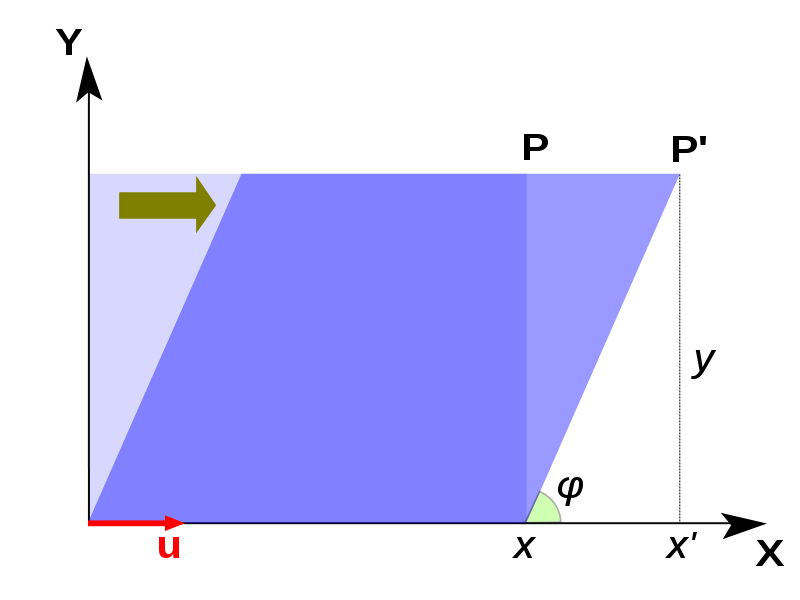
\includegraphics[width=0.4\textwidth]{plaatjes/shear}
%     \caption{Shear transformation. \cite{shear-fig}}
%     \label{fig:shear}
% \end{figure}%

% These transformations are applied by multiplying every point in a figure by a matrix built for that specific operation. This method can be used for operations as scaling, translations, rotations and shearing by creating a matrix which specifies each transformation in the following manner: 
% $\bigl(
%     \begin{smallmatrix}
%         x-scaling & shear-angle & x-translation \\ 
%         rotation & y-scaling & y-translation
%     \end{smallmatrix} 
% \bigr)$
% . In this case only shearing will be applied, and that is accomplished by using the matrix displayed in Equation \ref{eq:shear-matrix}. 

% \begin{equation}
%     \begin{pmatrix}
%         x' \\
%         y'
%     \end{pmatrix}
%     =
%     \begin{pmatrix}
%         1 & -a & 0 \\
%         0 & 1 & 0
%     \end{pmatrix}
%     \begin{pmatrix}
%         x \\
%         y
%     \end{pmatrix}
%     \label{eq:shear-matrix}
% \end{equation}

% The x and y-scaling values are set to $1$ to prevent any modification in the size of the image, and the $a$ value is the angle calculated using the PCA algorithm but negative to reverse the slant angle. Applying this affine transformation to the characters of the plate in Figure \ref{fig:slanted-plate} results in Figure \ref{fig:unslanted-plate}.

% \begin{figure}[ht]
%         \centering
%         \begin{subfigure}{0.33\textwidth}
%             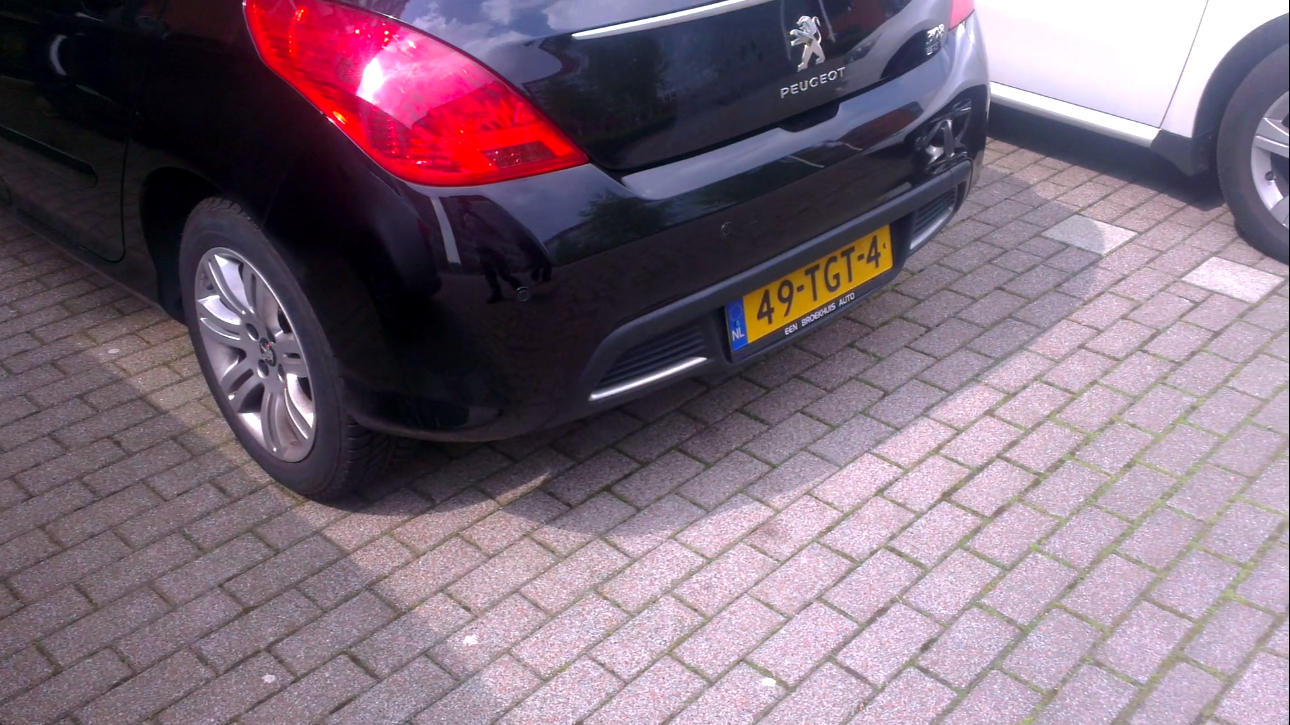
\includegraphics[width=\textwidth]{plaatjes/skewed-car}
%             \caption{Slanted plate source image.}
%             \label{fig:skewed-car}
%         \end{subfigure}%
%         ~ 
%         \begin{subfigure}{0.33\textwidth}
%             
\includegraphics[width=\textwidth]{plaatjes/slanted-plate}
%             \caption{Slanted plate characters.}
%             \label{fig:slanted-plate}
%         \end{subfigure}%
%         ~ 
%         \begin{subfigure}{0.33\textwidth}
%             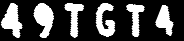
\includegraphics[width=\textwidth]{plaatjes/unslanted-plate}
%             \caption{Unslanted plate characters.}
%             \label{fig:unslanted-plate}
%         \end{subfigure}%

%         \caption{Process to unslant characters.}
%         \label{fig:unslanting-plate}
% \end{figure}

After this whole process, the plate is now ready to have the OCR software applied to it.

\paragraaf{Text recognition}

Although the Tesseract library works really well most of the time, it requires some training in some specific cases. The text displayed on license plates is one of those cases because it uses an unique font designed specifically to be used on plates. There is no official version of this font publicly available, but using LeFly's \cite{lefly} interpretation it was possible to train Tesseract to recognize this type of text. The font used for the training can be seen in Figure \ref{fig:plate-font}. Not every character has been added to the training text simply because not every character is used in license plates. The reasons for this ranges from characters being reserved for special plates, e.g. the royal family or diplomats, to characters that are too alike, e.g. the `I' and the `1' or `O' and the `0'.

\begin{figure}[ht]
    \centering
    
\includegraphics[width=0.8\textwidth]{plaatjes/font}
    \caption{License plate font.}
    \label{fig:plate-font}
\end{figure}%

Using the image displayed above and the external tools provided by the Tesseract library, training data can be generated. Tesseract does this by segmenting every item on the image and creating a file with its best guess at which character is represented on the image, its location on the image, and its size. This data is displayed in Figure \ref{fig:text-data}. After this file has been checked for possible mistakes, it can then be used to generated further necessary files where information on the shape of the characters, etc. are stored. Finally all the data is then bundled into a single file which can later be used with the recognition software.

\begin{figure}[H]
    \centering
    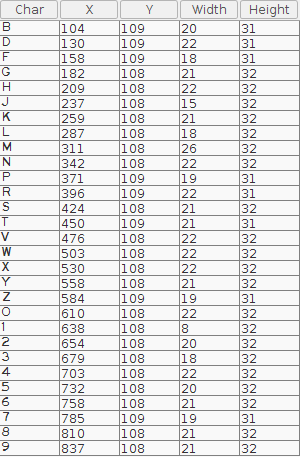
\includegraphics[width=0.3\textwidth]{plaatjes/text-data}
    \caption{Font data.}
    \label{fig:text-data}
\end{figure}%

Now if Tesseract is applied to the plate in Figure \ref{fig:unslanted-plate} using this training data, the results will be much better than without it.

\paragraaf{Database matching}

Once the plate has been found and the text has been parsed, the only thing left to do is to see if it's one of the cars the application is looking for. This component consists of two separate parts: matching the parse text with the database and updating the database.

First the application must retrieve a list with information about license plates of cars which are being searched for. Without this step it won't be possible to match the parsed text. This list is retrieved from a specific website using an HTTP socket. The website used for this application was a local dummy website. The information was stored in the JavaScript Object Notation (JSON) format. This is a simple way of storing and sending information objects between servers and clients. Once the information was retrieved from the website, it is stored in a file on the smartphone's storage. This process runs on a timer, which repeats itself after a specified amount of time, 30 minutes being the default.

The second part of this component is very simple. Once the text has been parsed, the application runs the parsed information through the database looking for a match. If a match is indeed found, the application will then retrieve the current GPS location and bundle it together with the plate information and the current time in a new JSON object and will the send it again via a HTTP socket. An example of a JSON annotation is displayed in Figure \ref{fig:json}.

\begin{figure}
    \begin{lstlisting}[language=json]
    { 
        "Plate": "XX-123-Y",
        "Date": "01-01-1970 00:00",
        "Latitude": "76.92061352",
        "Longitude": "41.04492187" 
    }
    \end{lstlisting}
    \caption{JSON annotation example}
    \label{fig:json}
\end{figure}

% #####################################################################################################################################################################################
\hoofdstuk{Validation}
% #####################################################################################################################################################################################

To define where the strengths and weaknesses of the software lie, some validation tests must be performed. These tests will provide information which will in turn be used to answer the research questions stated at the beginning of this thesis and, by extension, draw a conclusion on whether the project was successful. These test would be focused on three elements: the maximum distance and angle at which the application will give reliable results and how well does it perform while in a driving car.

\paragraaf{Distance}%

The validation based on the distance was tested on 4 different distances, 3, 4, 5 and 6 meters, while standing straight in front of the vehicle. The results are displayed in Figure \ref{fig:distance-test}. On Figure \ref{fig:3m-0a}, the text recognised is rather sharp and the OCR software has absolutely no problem parsing it. But the further away we go, the less and less sharp the text gets. Figures \ref{fig:4m-0a} and \ref{fig:5m-0a} still look clear and are parsed well, but once we get to the around 6 meters of Figure \ref{fig:6m-0a} the parsed text starts getting some inconsistencies. Although it might still be possible the application will parse the text correctly, more often than not it will return incorrect results. The maximum reliable distance lies therefore between 5 and 6 meters. %

% \clearpage

\begin{figure}[ht]
        \centering
        \begin{subfigure}{0.5\textwidth}
            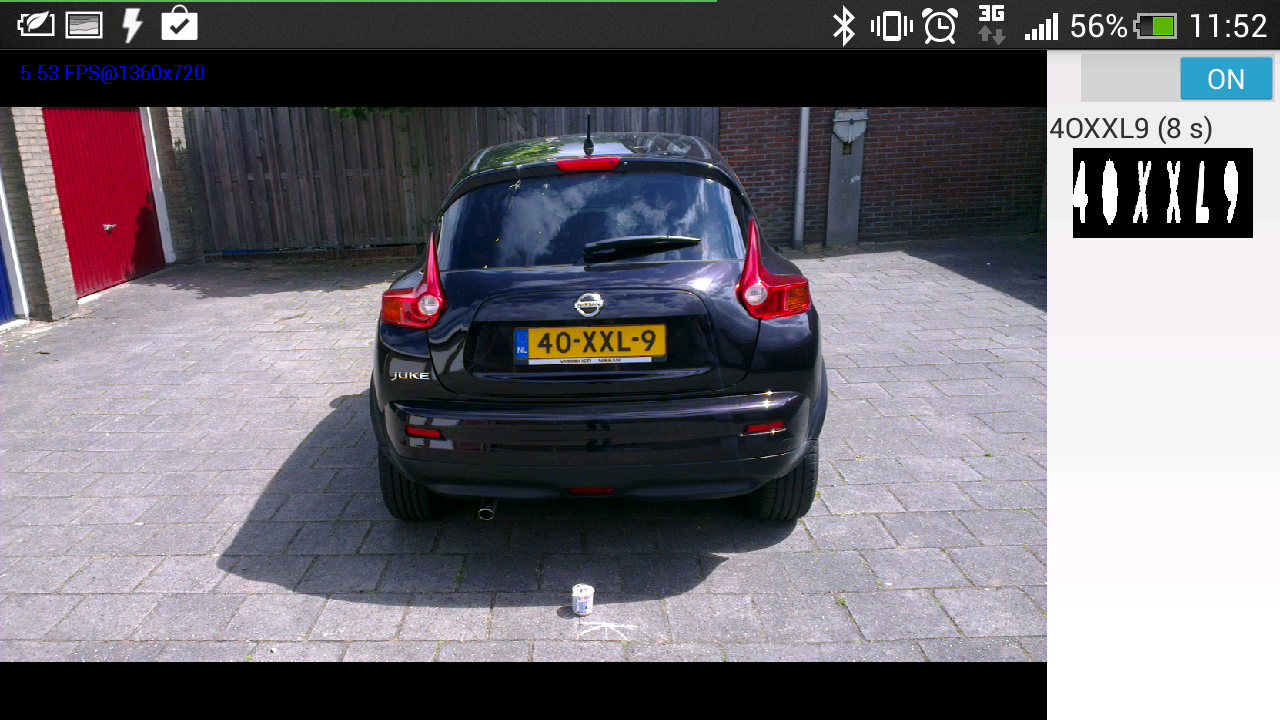
\includegraphics[width=\textwidth]{plaatjes/test-3m-0a}
            \caption{Vehicle at 3 meters, 0$^{\circ}$.}
            \label{fig:3m-0a}
        \end{subfigure}%
        ~ 
        \begin{subfigure}{0.5\textwidth}
            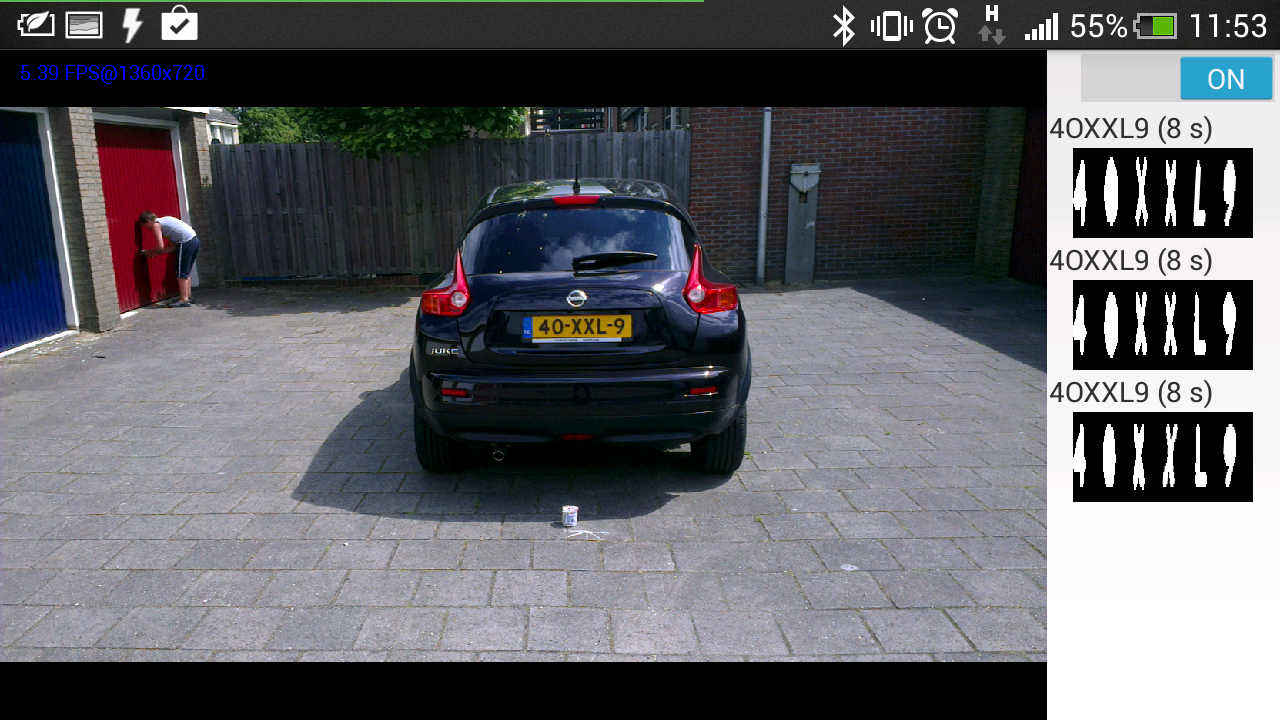
\includegraphics[width=\textwidth]{plaatjes/test-4m-0a}
            \caption{Vehicle at 4 meters, 0$^{\circ}$.}
            \label{fig:4m-0a}
        \end{subfigure}%
        % ~ 

        \begin{subfigure}{0.5\textwidth}
            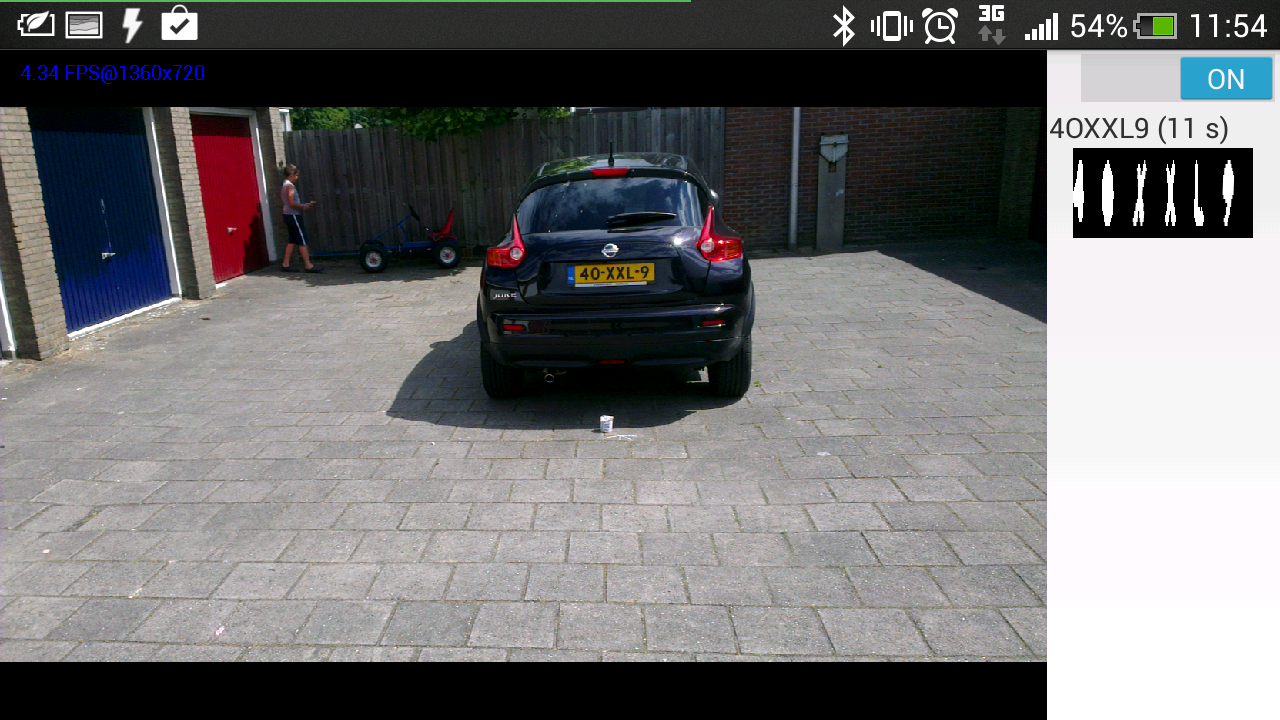
\includegraphics[width=\textwidth]{plaatjes/test-5m-0a}
            \caption{Vehicle at 5 meters, 0$^{\circ}$.}
            \label{fig:5m-0a}
        \end{subfigure}%
        ~
        \begin{subfigure}{0.5\textwidth}
            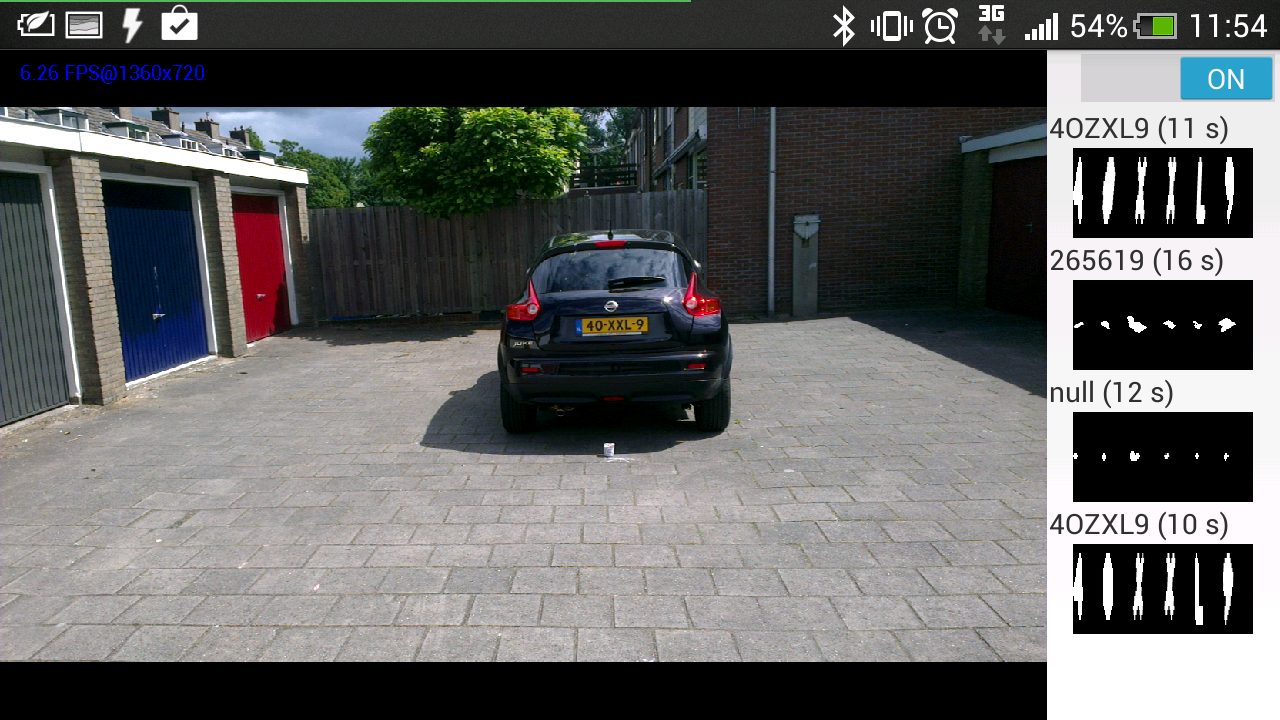
\includegraphics[width=\textwidth]{plaatjes/test-6m-0a}
            \caption{Vehicle at 6 meters, 0$^{\circ}$.}
            \label{fig:6m-0a}
        \end{subfigure}%

        \caption{Results at varied distances.}
        \label{fig:distance-test}
\end{figure} %

\paragraaf{Angle}

For the maximum angle test, angles were tested in an incremental way. Starting at the 6 meter 0$^{\circ}$ mark, because 6 meters was the last position the application worked, a small step was continuously taken in a circle around the vehicle and the application was tested. If no angle worked at this distance, the same was then repeated at a closer distance. By repeating this process, the boundary of the reliable working area was found. As shown in Figure \ref{fig:4m-47.5a}, the application was able to parse the text correctly, but in Figure \ref{fig:4m-47.5a-more} which is only a step further to the right, the application didn't work correctly. This point was located at a distance of 4 meters from the car and at an angle around 47,5$^{\circ}$.

\begin{figure}[H]
        \centering
        \begin{subfigure}{0.50\textwidth}
            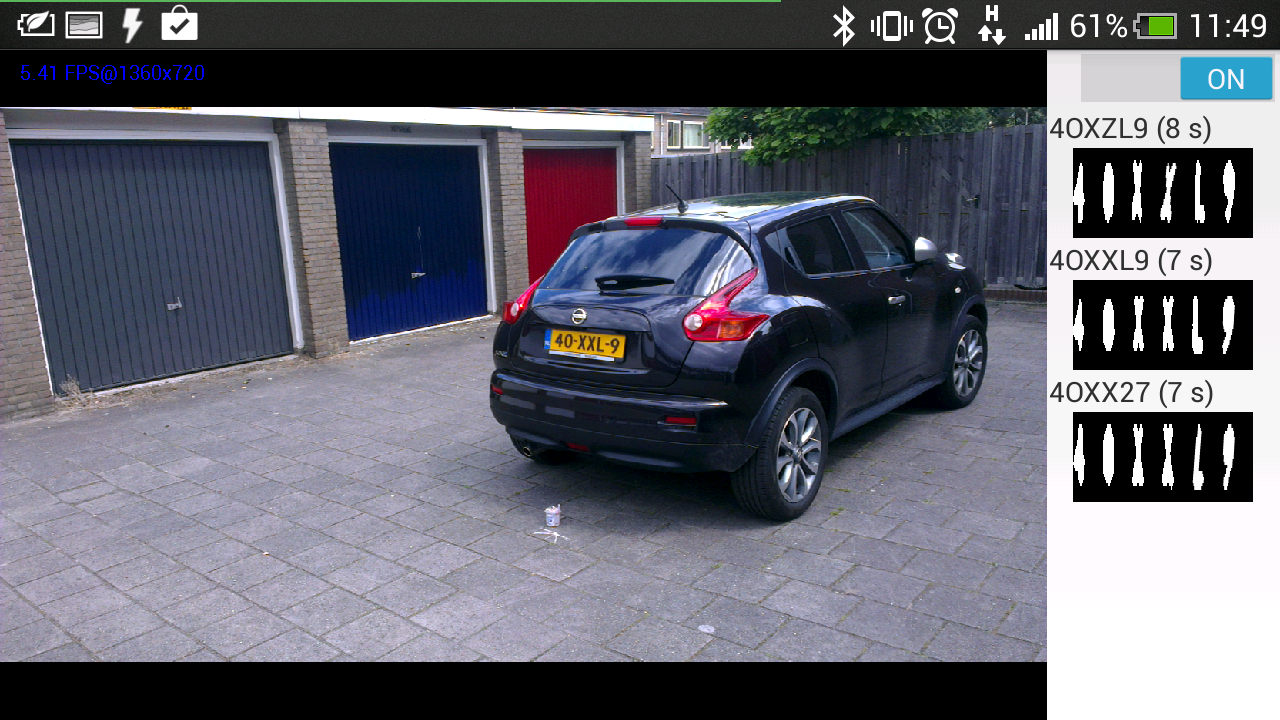
\includegraphics[width=\textwidth]{plaatjes/test-4m-47,5a}
            \caption{Vehicle at 4 meters, 47,5$^{\circ}$.}
            \label{fig:4m-47.5a}
        \end{subfigure}%
        ~ 
        \begin{subfigure}{0.50\textwidth}
            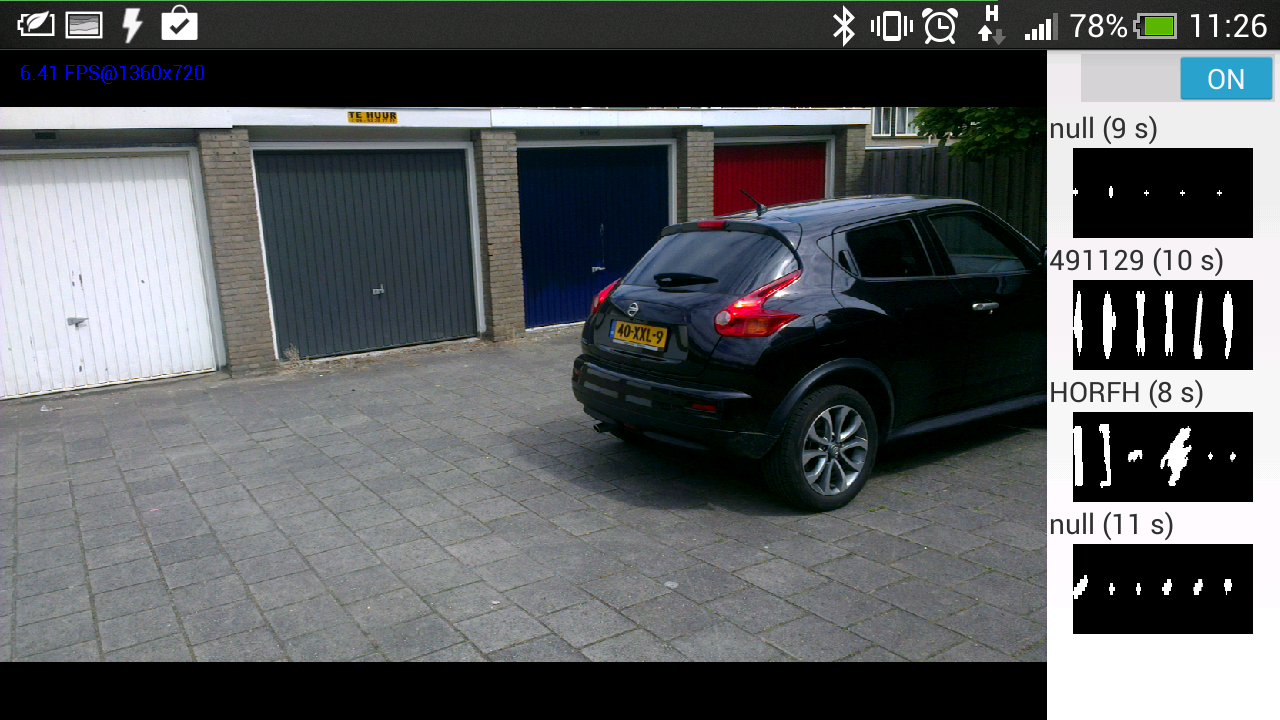
\includegraphics[width=\textwidth]{plaatjes/test-4m-47,5a+}
            \caption{Vehicle at 4 meters, \textgreater 47,5$^{\circ}$.}
            \label{fig:4m-47.5a-more}
        \end{subfigure}%
        % ~ 

        \caption{Results at varied angles.}
        \label{fig:angle-test}
\end{figure}%

\paragraaf{Text recognition}

To find out how well the text recognition work, images from different scenarios are used to test. One of the problems that haunt text recognition are characters that are similar in shape and this application is no stranger to that kind of problem. Even though most similar characters have been removed from license plates, i.e. the `0' and the `O', there are still characters that look similar enough when the plate is far away or at a difficult angle. For example, in Figure \ref{fig:real-scenario-1} the character `S' is continuously recognized as the number `5' because of the shape similarity, or in Figures \ref{fig:6m-0a} and \ref{fig:4m-47.5a-more} the character `X' is recognized as a `Z' because of the distance or angle of the image. 

\paragraaf{Real scenario}

Once the limitations of the application have been found, this data must be tested on a real scenario to see how well the application handles real usage. In Figure \ref{fig:real-scenario-1} the application is able to find the plate perfectly and parse the text almost correctly, because the vehicle is within the maximum distance and angle discovered in the sections above. In Figures \ref{fig:real-scenario-2} and \ref{fig:real-scenario-3} the application is not able to find the plates and much less parse the text because the plates are too far and/or too blurred. These limitations are related to the frame rate and resolution at which the video is captured and are not a direct limitation of the application itself. Possible solutions for the problems discovered in this chapter are discussed in the recommendations chapter.
\begin{figure}[H]
        \centering
        \begin{subfigure}{0.50\textwidth}
            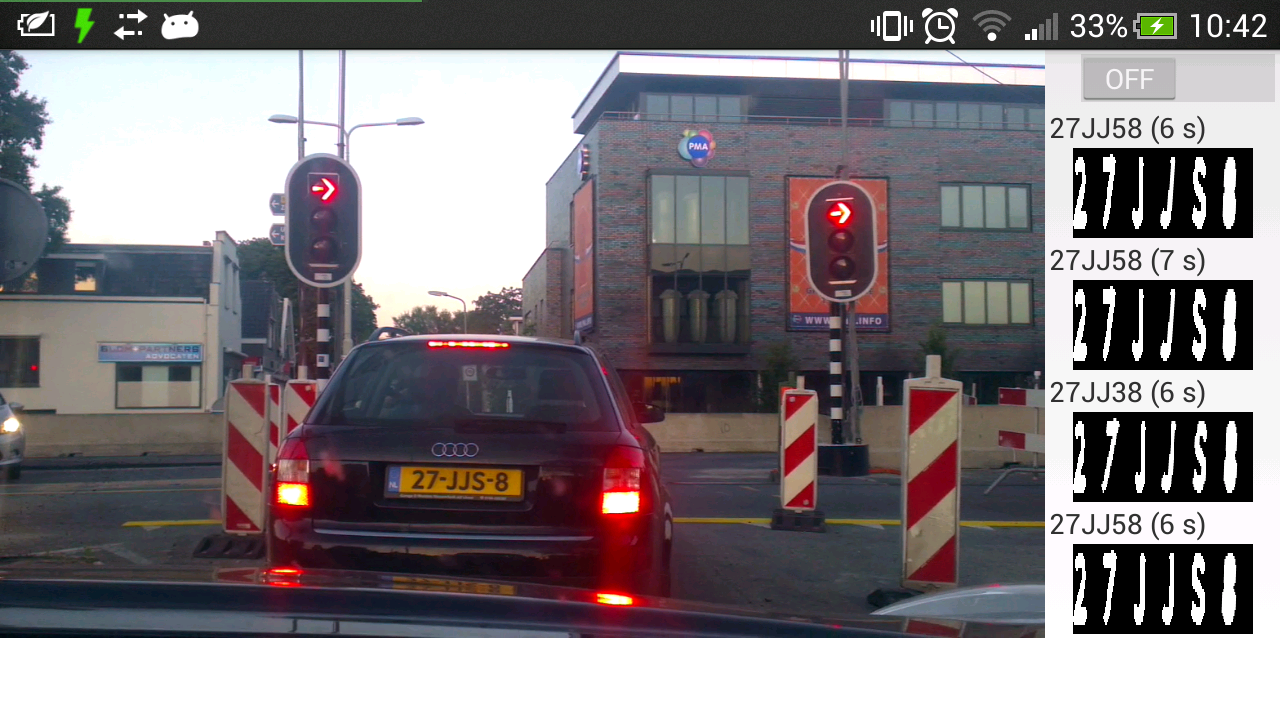
\includegraphics[width=\textwidth]{plaatjes/real-scenario-1}
            \caption{Vehicle at 4 meters, 47,5$^{\circ}$.}
            \label{fig:real-scenario-1}
        \end{subfigure}%
        ~ 
        \begin{subfigure}{0.50\textwidth}
            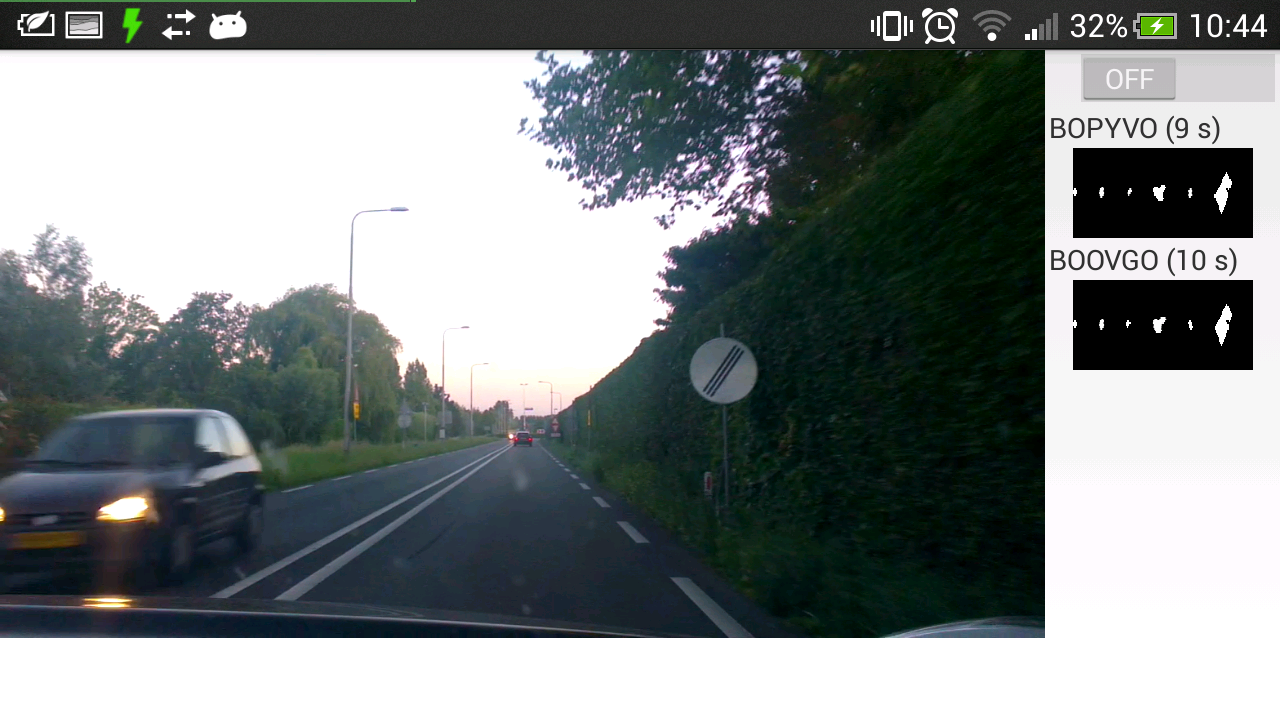
\includegraphics[width=\textwidth]{plaatjes/real-scenario-2}
            \caption{Vehicle at 4 meters, \textgreater 47,5$^{\circ}$.}
            \label{fig:real-scenario-2}
        \end{subfigure}%
        % ~ 

        \begin{subfigure}{0.50\textwidth}
            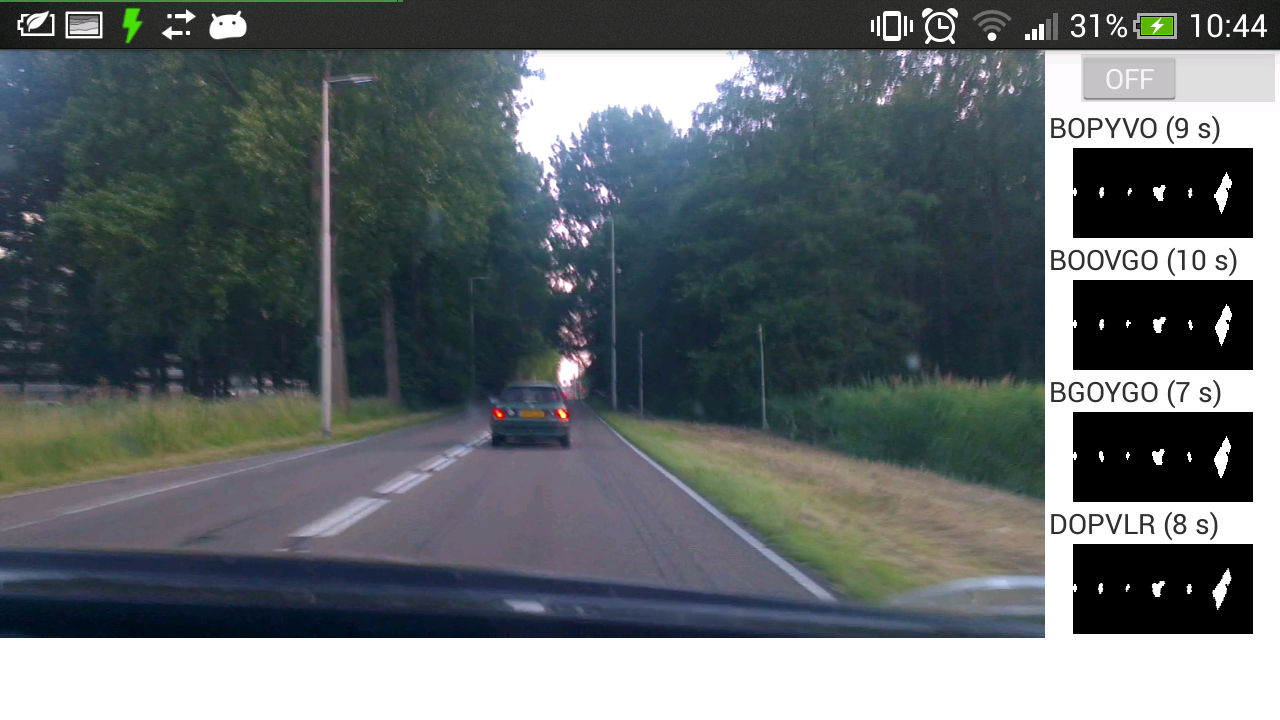
\includegraphics[width=\textwidth]{plaatjes/real-scenario-3}
            \caption{Vehicle at 4 meters, \textgreater 47,5$^{\circ}$.}
            \label{fig:real-scenario-3}
        \end{subfigure}%

        \caption{Results at varied angles.}
        \label{fig:real-scenario}
\end{figure}%
